\subsection{Das Kano-Modell}\label{subsec:kano-modell}
Für eine erfolgreiche Anforderungsanalyse ist es notwendig die Anforderungen an die Anwendung nicht nur zu erfassen,
sondern diese auch zu kategorisieren.
Dies ermöglicht es bei der anschließenden Entwicklung des Systems Anforderungen nach ihrer Priorität abzuarbeiten.
Im Rahmen dieser Arbeit wurde das Kano-Modell verwendet, um die erhobenen Anforderungen zu kategorisieren.
Wie Abbildung~\nameref{fig:kano_model} zeigt handelt es sich um ein Modell, welches die Erfüllung von Anforderungen mit
der Kundenzufriedenheit in Beziehung setzt.

\begin{figure}[ht]
    \centering
    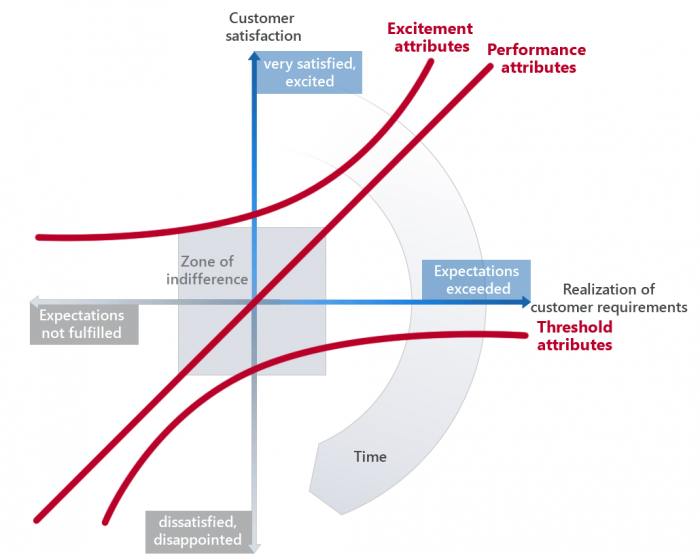
\includegraphics[width=0.8\textwidth]{images/Kano-Model}
    \caption{Kano-Modell~\autocite{kano-model}}
    \label{fig:kano_model}
\end{figure}

Die Anforderungen werden dabei in fünf Kategorien eingeteilt:

\begin{itemize}
    \item \textbf{Basisfaktoren:} Werden als selbstverständlich angesehen und führen bei fehlender Umsetzung für Unzufriedenheit
    \item \textbf{Leistungsfaktoren:} Werden vom Stakeholder explizit gefordert und führen zu Zufriedenheit bei Umsetzung
    und Unzufriedenheit bei Nichtumsetzung
    \item \textbf{Begeisterungsfaktoren:} Werden nicht explizit vom Stakeholder gefordert und führen auch nicht zu Unzufriedenheit
    bei Nichtumsetzung, steigern jedoch die Zufriedenheit bei Umsetzung
    \item \textbf{Gleichgültige Qualitäten:} Haben weder einen positiven noch einen negativen Einfluss auf die Kundenzufriedenheit,
    egal ob sie umgesetzt werden oder nicht
    \item \textbf{Umgekehrte Qualitäten:} Führen zu Unzufriedenheit bei Umsetzung aber nicht zu Zufriedenheit bei Nichtumsetzung
\end{itemize} (vgl.~\autocite{kano-model})
Wichtig zu beachten ist der Einfluss der Zeit auf die Kategorisierung der Anforderungen, denn mit fortschreitender Zeit werden
aus Begeisterungsfaktoren Leistungsfaktoren und aus Leistungsfaktoren Basisfaktoren.

\subsection{Anforderungsermittlung}\label{subsec:anforderungsermittlung}
Um Anforderungen kategorisieren zu können, müssen diese allerdings zuerst ermittelt werden.
Hierfür gibt es verschiedene Techniken, welche im Allgemeinen in folgende Kategorien eingeteilt werden können:

\begin{itemize}
    \item \textbf{Befragungstechniken:} Werden in direkter Zusammenarbeit mit dem Stakeholder durchgeführt (z.B.: Interviews, Fragebögen)
    \item \textbf{Kreativtechniken:} Entwicklung innovativer Ideen oder einer ersten groben Lösung (z.B.: Brainstorming, Perspektivenwechsel)
    \item \textbf{Dokumenten- und systembasierte Techniken:} Untersuchung bereits existierender Dokumente und Systeme,
    welche für die Anwendung relevant sind (z.B.: Systemarchäologie
    \item \textbf{Beobachtungstechniken:} Beobachtung der Stakeholder und ihrer Arbeitsabläufe (z.B.: Feldbeobachtung))
    \item \textbf{Unterstützende Techniken:} Werden ergänzend zu anderen Techniken angewandt (z.B.: Prototyping, Workshops)
\end{itemize} (vgl.~\autocite{Maulhardt.b})

In Kombination mit dem Kano-Modell kommen häufig Befragungstechniken und Kreativtechniken zum Einsatz.
Befragungstechniken ermöglichen es in Zusammenarbeit mit dem Stakeholder Anforderungen zu ermitteln und direkt nach dem
Kano-Modell zu kategorisieren,
und sind damit speziell für die Ermittlung der Leistungsfaktoren geeignet.
Kreativtechniken eignen sich hingegen besonders gut für die Ermittlung von Begeisterungsfaktoren, da diese nicht explizit
von den Stakeholdern gefordert werden.